\documentclass[prl,aps,twocolumn,floatfix,amsmath,amssymb,superscriptaddress,tightenlines]{revtex4}
\usepackage{graphicx}
%\usepackage{epstopdf}
\usepackage{amsfonts}
\usepackage{bm}
\usepackage{color}
\begin{document}

\date{\today}
\title{Measuring Renyi Entanglement Entropy with Quantum Monte Carlo}

%\author{Ann B. Kallin}
%\affiliation{Department of Physics and Astronomy, University of Waterloo, Ontario, N2L 3G1, Canada} 
%
%\author{Iv\'an Gonz\'alez}
%\affiliation{Centro de Supercomputaci\'on de Galicia, Avda.~de~Vigo~s/n, E-15705 Santiago de Compostela, Spain}
%
%\author{Matthew B. Hastings}
%\affiliation{Microsoft Research, Station Q, CNSI Building, University of California, Santa Barbara, CA, 93106}
%
%\author{Roger G. Melko}
%\affiliation{Department of Physics and Astronomy, University of Waterloo, Ontario, N2L 3G1, Canada} 

\begin{abstract} 
We develop a procedure for measuring the entanglemenet entropy of a region $A$ in a quantum
many-body system using valence-bond basis quantum Monte Carlo simulations.  Specifically, an 
estimator for the so-called Renyi $\alpha$-entropy, with $\alpha = 2$, is related to the expectation of
a unitary operator which swaps the basis states of a region $A$ with an ancillary copy of that region.
We demonstrate that the Renyi entropy calculated for a Heisenberg model in quantum Monte Carlo 
converges to exact results provided by density matrix renormalization group calculations.  Finally, we 
calculate the scaling of the Renyi entropy in the 2D Heisenberg model and confirm that the N\'eel 
groundstate obeys the expected area law.
\end{abstract}
\maketitle

{\it Introduction.}-- 
The measurement of entanglement in interacting quantum many-body systems has promised to provide
new tools and insight to the field of condensed-matter physics.  Most exciting are proposals to use 
entanglement as a probe to detect topological order, for example in paramagnetic spin liquids with no 
local order parameters, and fractional quantum hall states important in proposals for topologically protected qbits.  
A variety of measures of entanglement entropy are used, including fidelity, concurrence, and entropy, the 
latter being perhaps the most widely studied.  The general belief is that in two dimensions (2D) and higher, the 
leading contribution to the entanglement entropy scales as the boundary of a subsystem $A$ -- the so-called
``area law''.  In additional to important corrections in topological phases, subleading universal corrections are
believed to occur in the presence of a quantum critical point, or because of the presence of ``corners'' in the region
$A$.  Thus, the study of entanglement entropy would provide a rich new avenue for the study of ...

A major obstacle in the use of entanglement entropy as a resource for studying condensed-matter systems is 
the difficulty in calculating it numerically in 2D and higher.

Consider the Renyi entropy, defined as 
\begin{equation}
S_{\alpha} (\rho_A) = \frac{1}{1- \alpha} \ln \left[{ {\rm Tr}\big( \rho_A^{\alpha} \big) }\right],
\end{equation}
where $\rho_A$ is the reduced-density matrix of a subregion $A$ entangled with its complement $B$, and 
$\alpha$ is a positive-definite integer parameter.  In the limit $\alpha \rightarrow 1$, one recovers the formal 
definition of the von Neumann entropy, $S_1 (\rho_A) = - {\rm Tr}( \rho_A \ln \rho_A )$.  The von Neumann entropy
is accessible numerically only in procedures where the reduced density matrix can be calculated directly, such as Lanczos 
or DMRG.  Scalable simulations methods in $D>1$, needed in order to study the groundstate, finite-temperature, and 
critical properties of the vast majority of systems of interested to condensed-matter physics, are so far essentially
restricted to quantum Monte Carlo (QMC).  However, the functional dependence of $\rho_A$ inside of the trace in the 
von Neumann makes calculating $S_1$ in QMC difficult or impossible.  

The general Renyi $\alpha$-entropies has recently attracted considerable attention, due to their ability to encode
information about the whole ``entanglement spectrum'' of $\rho_A$, together allowing the set of $S_{\alpha}$ to contain 
much more information that $S_1$ alone.  For example, the concept of topological entanglement entropy has recently been
generalized to the family of Renyi entropies, where it has been shown to be equal to the logarithm of the total quantum 
dimension, $S_{\rm top} \propto \log D$, regardless of $\alpha$ \cite{PI}.  Universal corrections to the scaling of $S_{\alpha}$ 
have also recently been calculated in a field-theoretic treatment of the $O(N)$ model \cite{Max}.
In addition, two Renyi entropies $S_{\alpha}$ and $S_{\beta}$ obey the fundamental
inequality $S_{\alpha} \geq S_{\beta}$ when $\alpha > \beta$, making for example $S_2$ useful as a rigorous
lower bound on $S_1$.  

In this paper we show that the Renyi entropy $S_2$ can be represented in the valence-bond basis as the expectation
value of a unitary swap operator.  This swap operator is directly accessible as a simple expectation value in a QMC simulation scheme
based on the valence-bond basis.  Using QMC simulations, we calculate the entropy $S_2$ for a $S=1/2$ Heisenberg model
in 1D and 2D lattices.  In 1D, we demonstrate that $S_2$ calculated with QMC converges to the exact result obtained with DMRG simulations.  In 2D, we show that the leading order term in the scaling of $S_2$ goes like the boundary of the region $A$, 
confirming the area law expected from recent studies \cite{Ann}.

\begin{figure} {
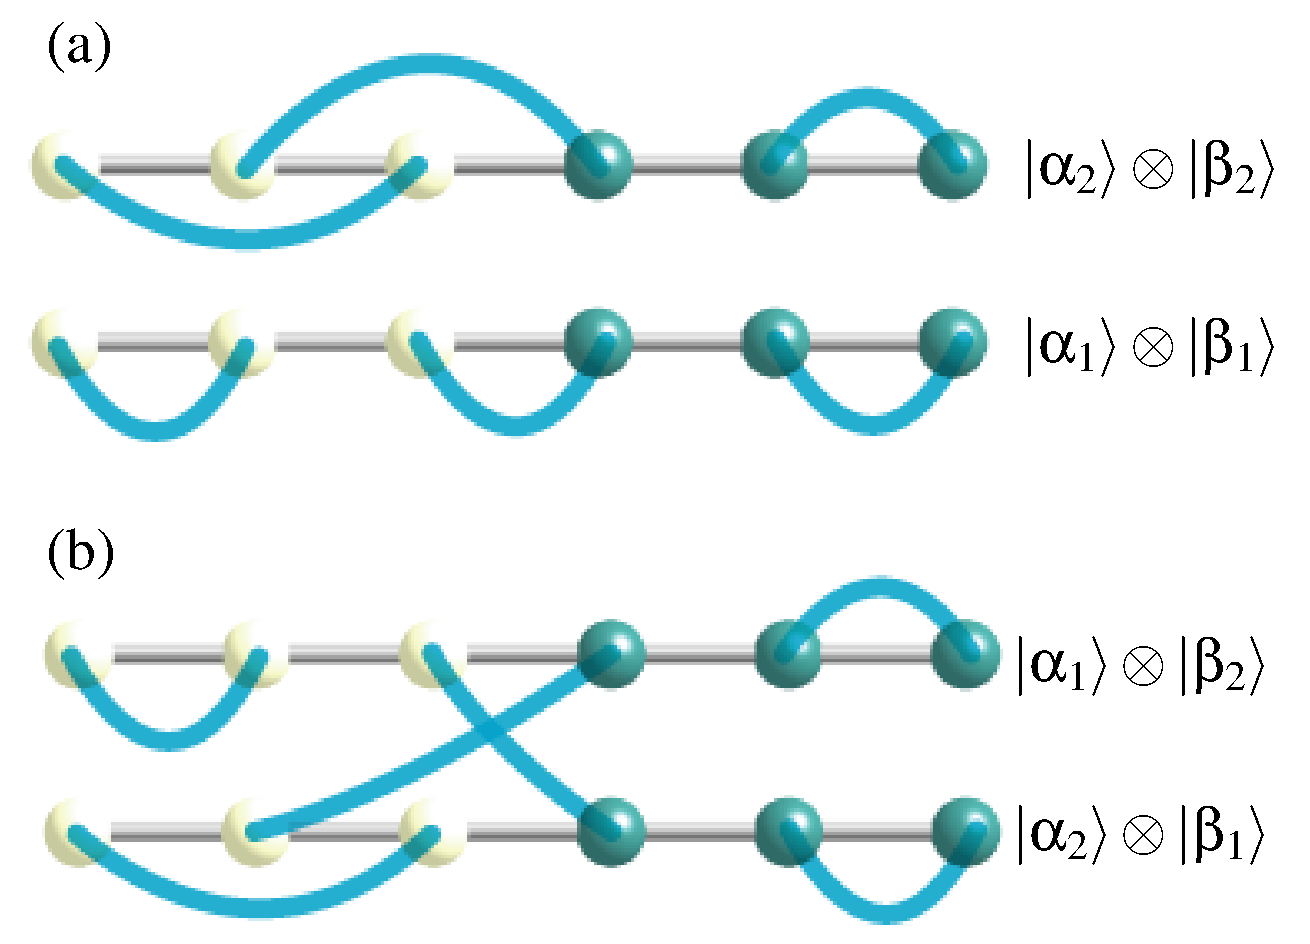
\includegraphics[width=2.5
in]{swap_2.eps} \caption{(color online) 
\label{swap_2}
A six-site chain, with two non-interacting copies (top and bottom) before (a) and after (b) operation of the $Swap_A$ operator.  
The region A consists of three light-colored sites on the left; the entangled region B of three dark sites on the right.
}
} \end{figure}

{\it Valence-bond basis and the Swap operator.}-- We follow the notation of Sandvik, and write the expansion of a singlet
wavefunction $\Psi$ of $N$ spins as $N/2$ valence bonds:
\begin{equation}
| \Psi \rangle = \sum_r f_r|(a^r_1,b^r_1) \ldots (a^r_{N/2},b^r_{N/2}) \rangle = \sum_r f_r| V_r \rangle
\end{equation}
where the valence bonds (singlet pairs) denoted by $(a,b) = (\uparrow_a \downarrow_b - \downarrow_a \uparrow_b)/\sqrt{2}$ occur between sites of the opposite sublattices of a bipartite lattice, and $r$ labels all possible tilings of bonds.  The coefficients $f_r$ are unknown, but an importance sampling scheme for the valence bond state $| V_r \rangle$ is outlined below.  

We now give an equivalent definition of
the Renyi entropy $S_2$ as the expectation
value of a {\it Swap} operator on two copies of the system.  
%We first
%present a formal solution to the problem of measuring the entropy
%in QMC, Eq.~(\ref{ensembleavg}) below, as a QMC averge.
%We then explain how to better perform the statistical sampling for
%actual calculations.
Define an
operator $Swap_A$ which acts on two copies of the system, swapping the
configurations within region $A$.  To more precisely define the operator
$Swap_A$, we now write out its matrix elements in a product basis.
Let $|\alpha\rangle$  represent a complete basis of states in region
$A$ and let $|\beta\rangle$ represent a complete basis of states in
region $B$.  Then, $|\alpha\rangle \otimes |\beta\rangle$ represent
a complete basis of states for the whole system, and
$\Bigl( |\alpha_1\rangle \otimes |\beta_1\rangle \Bigr) \otimes
\Bigl( |\alpha_2\rangle \otimes |\beta_2\rangle \Bigr)$
represent a complete basis of states for two copies of the system.
Define the operator $Swap_A$ by
\begin{eqnarray}
&& Swap_A \Bigl( |\alpha_1\rangle \otimes |\beta_1\rangle \Bigr) \otimes
\Bigl( |\alpha_2\rangle \otimes |\beta_2\rangle \Bigr) \nonumber \\ &&=
\Bigl( |\alpha_2\rangle \otimes |\beta_1\rangle \Bigr) \otimes
\Bigl( |\alpha_1\rangle \otimes |\beta_2\rangle \Bigr).
\end{eqnarray}
The operator $Swap_A$ is a unitary operator.
On immediately sees that the Renyi entropy is simply
\begin{eqnarray}
\label{H2fromSwap}
S_2(\rho_A) &=&-\ln(\langle \Psi\otimes \Psi|Swap_A|\Psi\otimes \Psi\rangle) \\
&=&-\ln(\langle Swap_A \rangle).
\end{eqnarray}
The $Swap_A$ operator is illustrated for a 1D lattice with six sites.  There, two copies of the system (``real'' and ``ancillary'') are
drawn before (a) and after (b) operation by the $Swap_A$ operator.  The result is an entangling of the valence bonds between the 
real and ancillary systems across the boundary of the region $A$.

{\it Measuring the Swap operator in QMC.}--
We now present a procedure for measuring the entropy $S_2$ via importance sampling of the $Swap_A$ operator in QMC.  A
projector scheme in the valence-bond basis has recently been popularized by Sandvik \cite{Sandvik}, where high powers of
a Hamiltonian $H$ are used to project out the ground state $|0\rangle$ from a trial wavefunction, 
$(-H)^m|\Psi \rangle \propto |0\rangle$.  In Sandvik's QMC scheme, $(-H)^m$ is written as a sum of all products of $m$ bond
operators,
\begin{equation}
(-H)^m = \sum_r \prod_{i=1}^m H_{a_i^r b_i^r} = \sum_r P_r,
\end{equation}
where for simplicity we use the Heisenberg model, defining $H=-\sum_{\langle a,b \rangle}H_{ab}$ and 
$H_{ab} = -({\bf S}_a \cdot {\bf S}_b - 1/4)$.  The operator string $P_r$ is sampled according to its weight, $W_r$, accrued upon
evolution of a trial valence-bond state $|V \rangle$ under projection:
\begin{equation}
P_r |V \rangle = W_r |V(r) \rangle.
\end{equation}
As shown in Ref.~\cite{Sandvik}, for the Heisenberg model, $W_r$ is simply related to the number of off-diagonal 
operations $m_{\rm off}$ in the projection, $W_r = 2^{-m_{\rm off}}$.

To sample the $Swap_A$ operator, one requires a double-projector valence-bond QMC scheme \cite{Sandvik}, where
a general expectation value for an observable $\mathcal{O}$ is given by
\begin{equation}
\label{expect}
\langle \mathcal{O} \rangle = \frac{\sum_{rl} \langle V | P_l^* \mathcal{O} P_r | V \rangle} {\sum_{rl} \langle V | P_l^* P_r | V \rangle} 
= \frac{\sum_{rl} W_l W_r \langle V(l) | \mathcal{O} | V(r) \rangle} {\sum_{rl} W_l W_r \langle V(l) | V(r) \rangle}
\end{equation} 
This expectation value can be applied directly to the $Swap_A$ operator, illustrated in Fig.~\ref{swap_2}.  Namely, one 
performs important sampling of operator strings according to the weight $W_l W_r \langle V(l) | V(r) \rangle$, and measures
the QMC average expectation value
\begin{equation}
\langle Swap_A \rangle =  \left\langle{ \frac{ \langle V(l) | Swap_A | V(r) \rangle}{\langle V(l) | V(r) \rangle}  }\right\rangle 
\end{equation}

\begin{figure} {
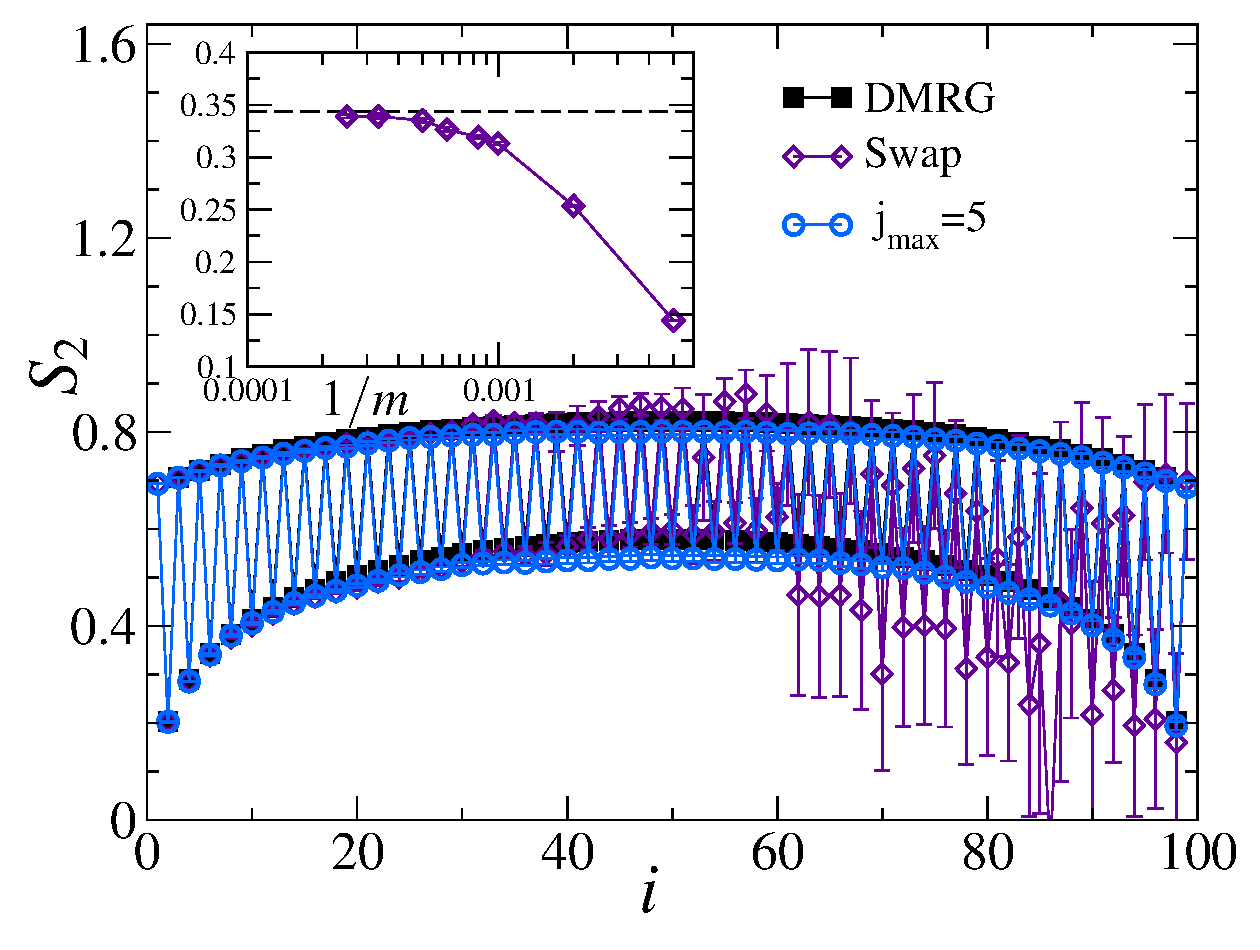
\includegraphics[width=2.8in]{L100_fig2.eps} \caption{(color online) 
\label{1Dfig}
The Renyi entropy $S_2(x)$ as a function of site index $x \in A$, for a 100-site Heisenberg chain with open boundaries, 
calculated with DMRG and QMC.  The data for $\langle Swap_A \rangle$ was obtained with one simulation, whereas ``Ratio'' labels data for 
${\langle Swap_{A^{i+j}}\rangle}/{\langle Swap_{A^{i}}\rangle}$
with a range of  $j \in [1,5]$.  The inset shows the convergence of $S_2(6)$ up to $m=4000$.
}
} \end{figure}

Results are illustrated in Fig.~XXX.  There, simulations were performed using a simple double-projector QMC \cite{Sandvik}, where
the trial $| V \rangle$ is a columnar state, four random bond operators were changed per Monte Carlo step, and unless otherwise
stated $m=40N$.  Exact results for $S_2(\rho_A)$ were obtained with a DMRG simulation, converged with 1000 states.  One 
immediately sees that the naive expectation value $\langle Swap_A \rangle$ results in a grossly incorrect result when the region
$A$ grows large (in 1D, $A$ is the linear region of size $x$).   
One may understand this by invoking the area law: namely,
we expect
that $S_2(\rho_A)$ will be proportional to the {\it surface area} of the region
$A$ (and in certain systems, such as one dimensional critical systems, it
may be even larger, of order the log of the interior size).  Thus,
the expectation value $\langle Swap_A \rangle$ should be exponentially small in the
surface area of $A$.  Thus once $A$ becomes
large, we are computing a very small quantity and
statistical fluctuations will be important;
%(it is not clear whether or not the numerator in the average
%of (\ref{ensembleavg}) should be positive for every given realization,
%though maybe it is; even if it is positive for every realization,
%so that we are averaging a positive quantity, 
the fact that the expectation
of $Swap_A$ is so small means that we are doing the importance sampling
incorrectly, since then only very few configurations contribute much to this
expectation value.

To combat this issue, we propose the following refinement to the algorithm: define regions $A^1,A^2,...,A^n$, such
that $A^i$ contains $i$ sites, and $A^i$ is a subset of $A^{i+1}$.  So, each region $A^{i+1}$ is obtained by adding one site to region
$A^{i}$, and region $A^0$ is the empty set (thus, $Swap_{A^0}$ is equal to the identity operator).
Then, if one computes the ratio
\begin{equation}
\frac{\langle Swap_{A^{i+1}}\rangle}{\langle Swap_{A^{i}}\rangle}
= \frac{\sum_{rl} W_l W_r \langle V(l) | Swap_{A^{i+1}} | V(r) \rangle} {\sum_{rl} W_l W_r \langle V(l) | Swap_{A^i} | V(r) \rangle}
\end{equation}
for each $i=0,...,n-1$, the log of this ratio is equal to minus the
difference $S_2(\rho_{A^{i+1}})-S_2(\rho_{A^{i}})$.
Computing this ratio for each $i$ will let us compute $S_2$ for all $A^i$.  To calculate this ratio, simulations must be performed 
with the modified sampling weight
\begin{equation}
W_l W_r \langle V(l) | Swap_{A^i} | V(r) \rangle,
\end{equation}
i.e., a unique QMC simulation must be performed for each desired $i$.  Thus, our simple double-projector algorithm, which scales 
approximately as $~{\rm max}(m^2, N)$ \cite{AWSloop}, obtains an additional multiplicative factor of $N$ in the scaling.  In practice, 
this can be reduced by noting that good statistical control can be retained by calculating 
${\langle Swap_{A^{i+j}}\rangle}/{\langle Swap_{A^{i}}\rangle}$ for a range of $j \in [1,j_{\max}]$.  We illustrate this in Fig.~\ref{1Dfig},
where simulations with $j_{\rm max}=5$ are sufficient to converge a 1D chain with $N=100$ to the exact results within error bars.

{\it 2D Heisenberg Results.}-- We now extend these concepts to QMC simulations of the spin 1/2 Heisenberg model on $N=L \times L$ lattices.  We define the entangled region $A$ as a square region of linear length $\ell$ encompassing $\ell \times \ell$ sites.  We calculate the expectation value of both the $\langle Swap_A \rangle$ directly using one simulation, as well as the ratio ${\langle Swap_{A^{\ell+r}}\rangle}/{\langle Swap_{A^{\ell}}\rangle}$.  Here, both $\ell$ and $r$ are variables denoting the linear dimension of $A$; i.e. $A^{\ell+r}$ contains $2(\ell+r)$ more sites than $A^{\ell}$.

\begin{figure} {
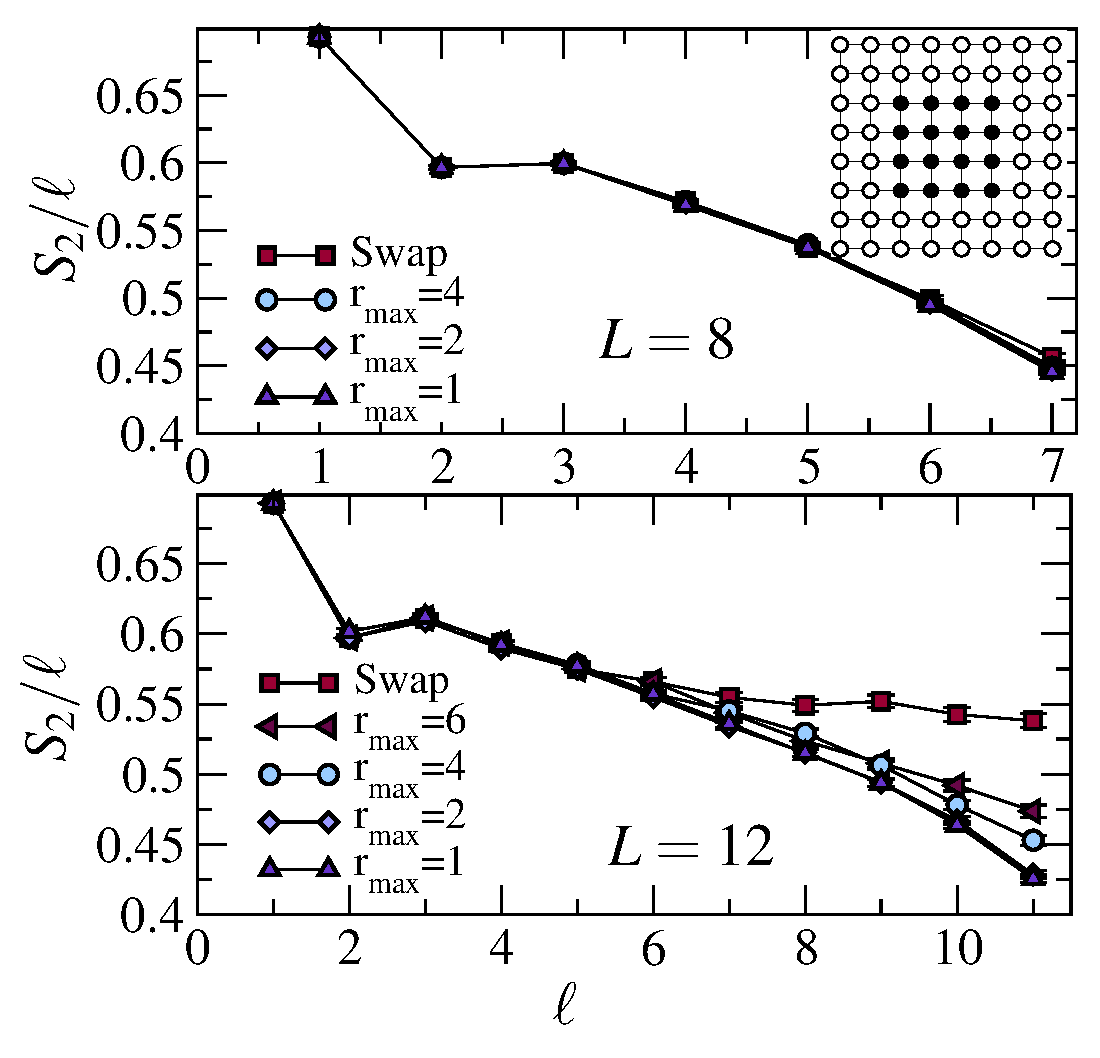
\includegraphics[width=2.8in]{L8n12_ratio.eps} \caption{(color online) 
\label{L16fig}
}
} \end{figure}

Figure \ref{L16fig} illustrates $S_2$ on a 2D $L=16$ Heisenberg model, which converges as one successively decreases the range of $r \in [1,r_{\rm max}]$ from $r_{\rm max}=16$, corresponding to one simulation of the bare $Swap_A$ estimator, to $r_{\rm max}=1$, which corresponds to 14 different simulations of the ratio estimator ${\langle Swap_{A^{\ell+r}}\rangle}/{\langle Swap_{A^{\ell}}\rangle}$.  It is important to note that for large $r_{\rm max}$ the correct value of $S_2$ does {\it not} lie within the error bars of the data.  This is an indication that the algorithm will not converge to the expected result in polynomial time, since the expectation value is exponentially decreasing.


\begin{figure} {
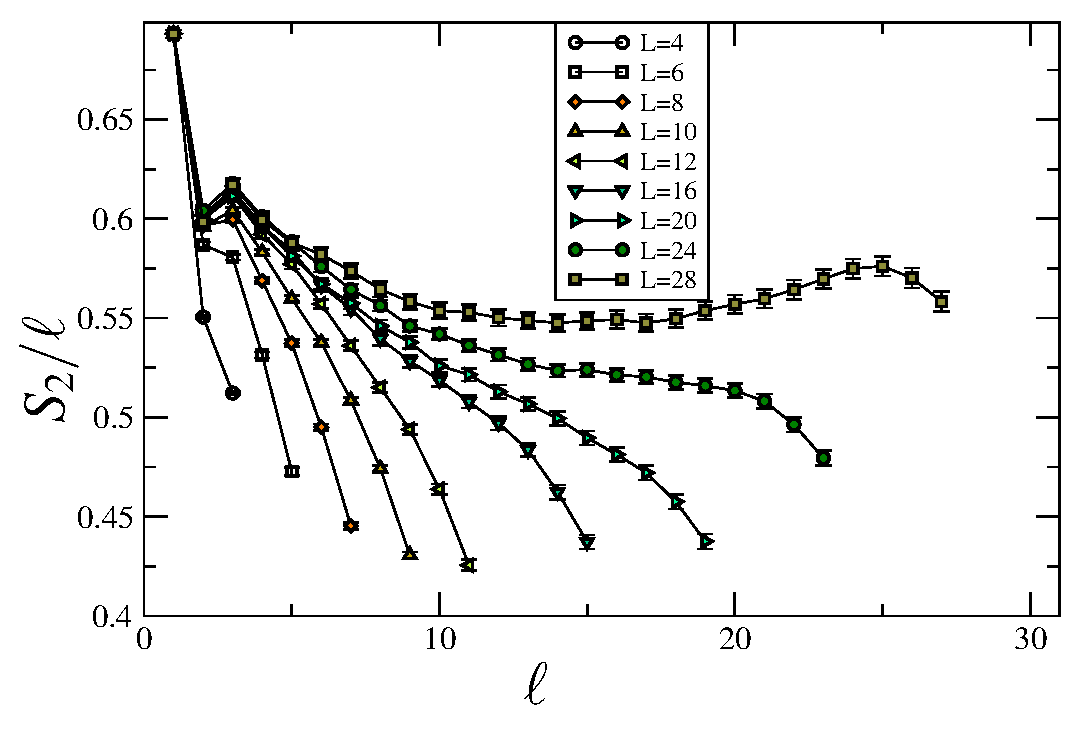
\includegraphics[width=3.1in]{fig4.eps} \caption{(color online) 
\label{fig4}
}
} \end{figure}



{\it Acknowledgments.}-- The authors thank ...
This work was made possible by the
computing facilities of SHARCNET and CESGA.  Support was provided by NSERC
of Canada (R.G.M.).

\bibliography{Biblio}

\end{document}
